\chapter{Arduino sensor specification and implementation}\label{cap:implementacion}

\section{Introduction}
There are infinitely many ways of implementing sensors in a computer system. Internet of things is slowly becoming a topic that people interested in technology are talking about. For our particular case, we will be using an Arduino MEGA 2560 board.

\begin{figure}[H]
    \centering
    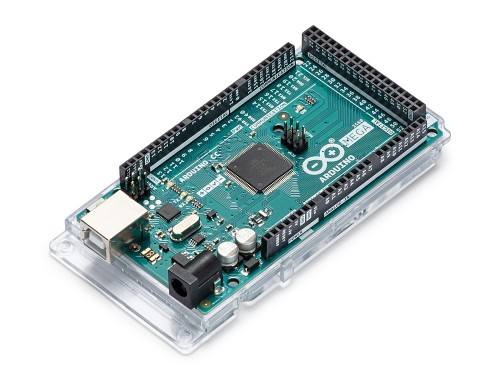
\includegraphics[width=0.5\textwidth]{fig/mega2560.jpg}
    \caption{Arduino MEGA 2560 board}
    \label{fig:mega2560}
\end{figure}



\section{Specifications}
Let's take a look at some of the options that the different sensors offer. In this section we will specify some sensors in order to understand what these components are capable of, then, we will implement the two of them that are considered to be more crucial in harvesting, since those are the ones that we are interested in for this prototype. 

We know we will be working with an Arduino MEGA 2560 board, but it goes without saying, we will also need some more components. 

\subsection{FC-28 Soil Moisture Sensor}
Soil moisture sensor is likely the main sensor when harvesting is concerned as it helps farmers manage their irrigation systems more efficiently. This won't only save water but will also increase the quality of the crops since it can control moisture to the milimeter at all diferent plant growth stages. In this section, we are going to be documenting the process of using the sensor FC-28 with our Arduino board.

\subsubsection{How does it work?}
This FC-28 hygrometer module consists of two probes that measure the volumetric content of water. The current passes through the soil, which gives the resistance value between the metallic probes and measures the moisture value. The reason why this works fine is simple: the more water a soil has, the more electricity will be conducted which means less resistance.

\begin{figure}[H]
    \centering
    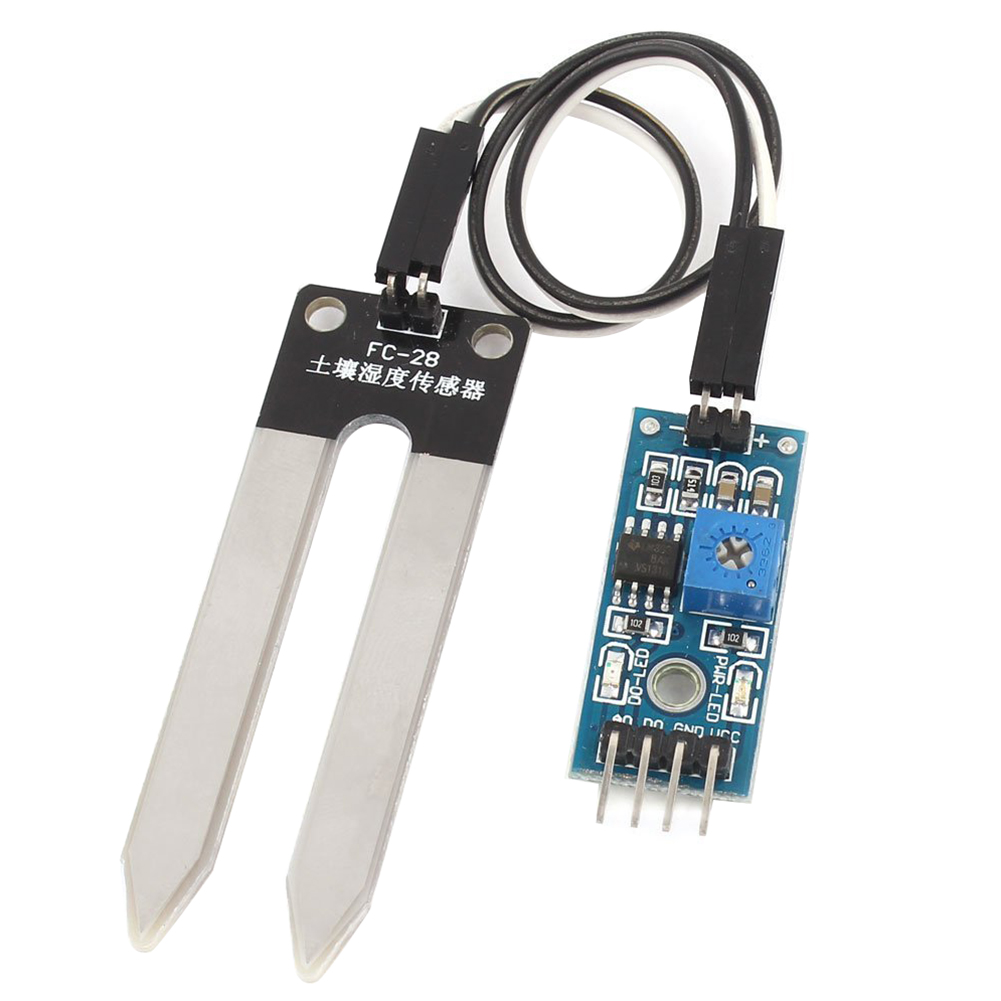
\includegraphics[width=0.35\textwidth]{fig/fc28.jpg}
    \caption{A FC-28 moisture sensor}
    \label{fig:fc28}
\end{figure}

Besides the sensor itself, there is another component that has two LEDs (one for output and another for power), a potentiometer and a LM293 comparator.

\subsubsection{Using the sensor}
The values that the sensor picks up goes from 0 to 1023. Ideally it would show 0 when sunken underwater and 1023 when is only in contact with the air, in other words, when it's not in contact with soil.

Let's implement a small script to understand the behaviour of the sensor. The circuit that we will be using is really simple:
\begin{itemize}
	\item The VCC of the FC-28 goes to 5V of the Arduino
	\item The GND of the FC-28 goes to GND of the Arduino
	\item The pin A0 of the FC-28 goes to the pin A0 of the Arduino
\end{itemize}
Here's a diagram of the circuit.

\begin{figure}[H]
    \centering
    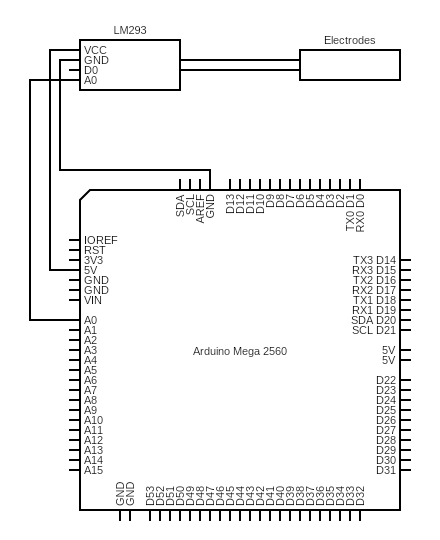
\includegraphics[width=0.5\textwidth]{fig/fc28-scheme-circuit.png}
    \caption{Diagram of the circuit for the FC-28}
    \label{fig:fc28-scheme-circuit}
\end{figure}


This is how circuit should look like once assembled.
	\begin{figure}[H]
		\centering
		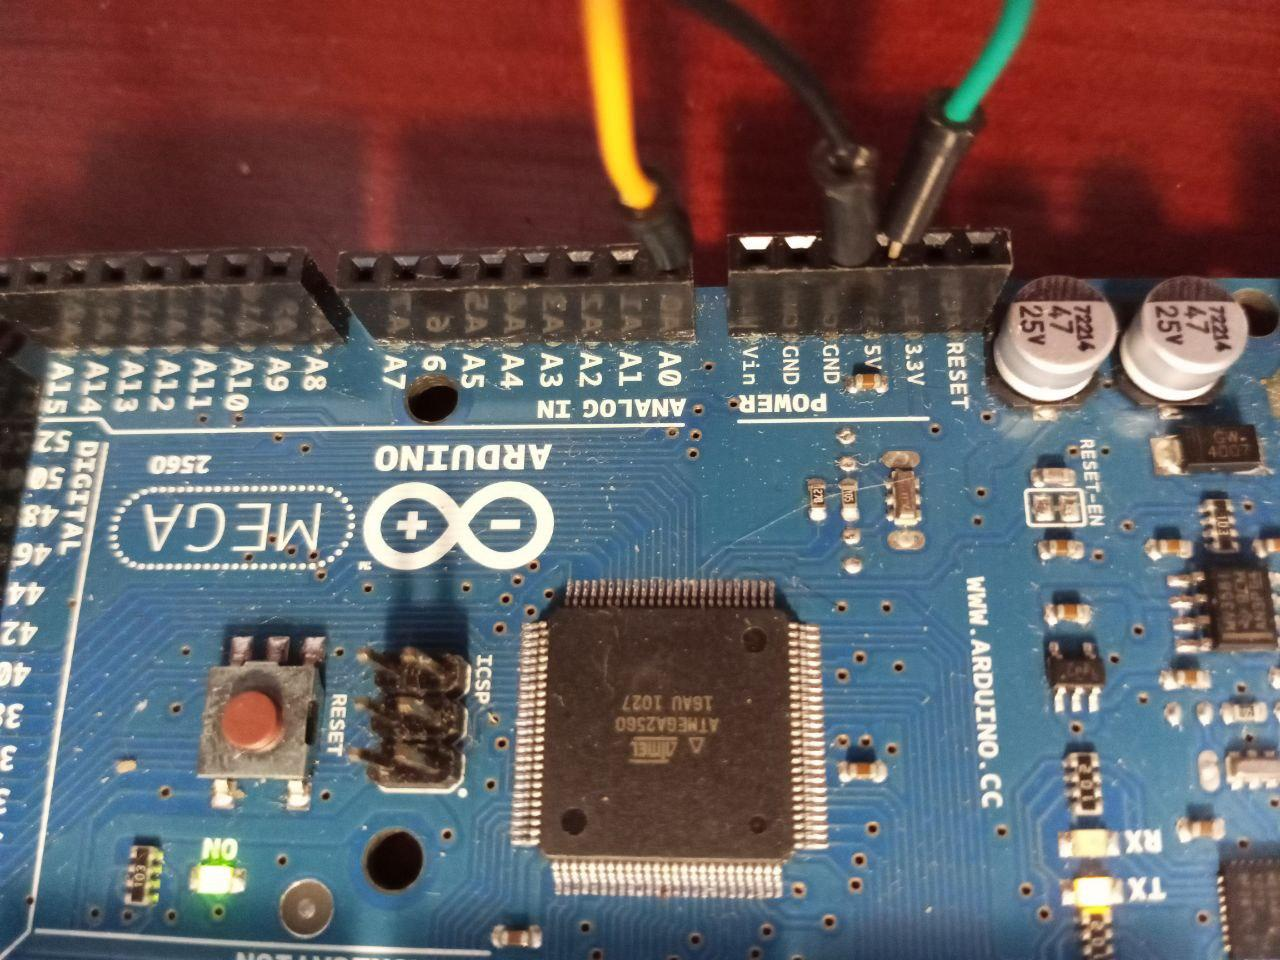
\includegraphics[width=0.35\textwidth]{fig/fc28-circuit1.jpg}
		\caption{Board for FC-28 connections}
	\end{figure}
	\hfill
	\begin{figure}[H]
		\centering
		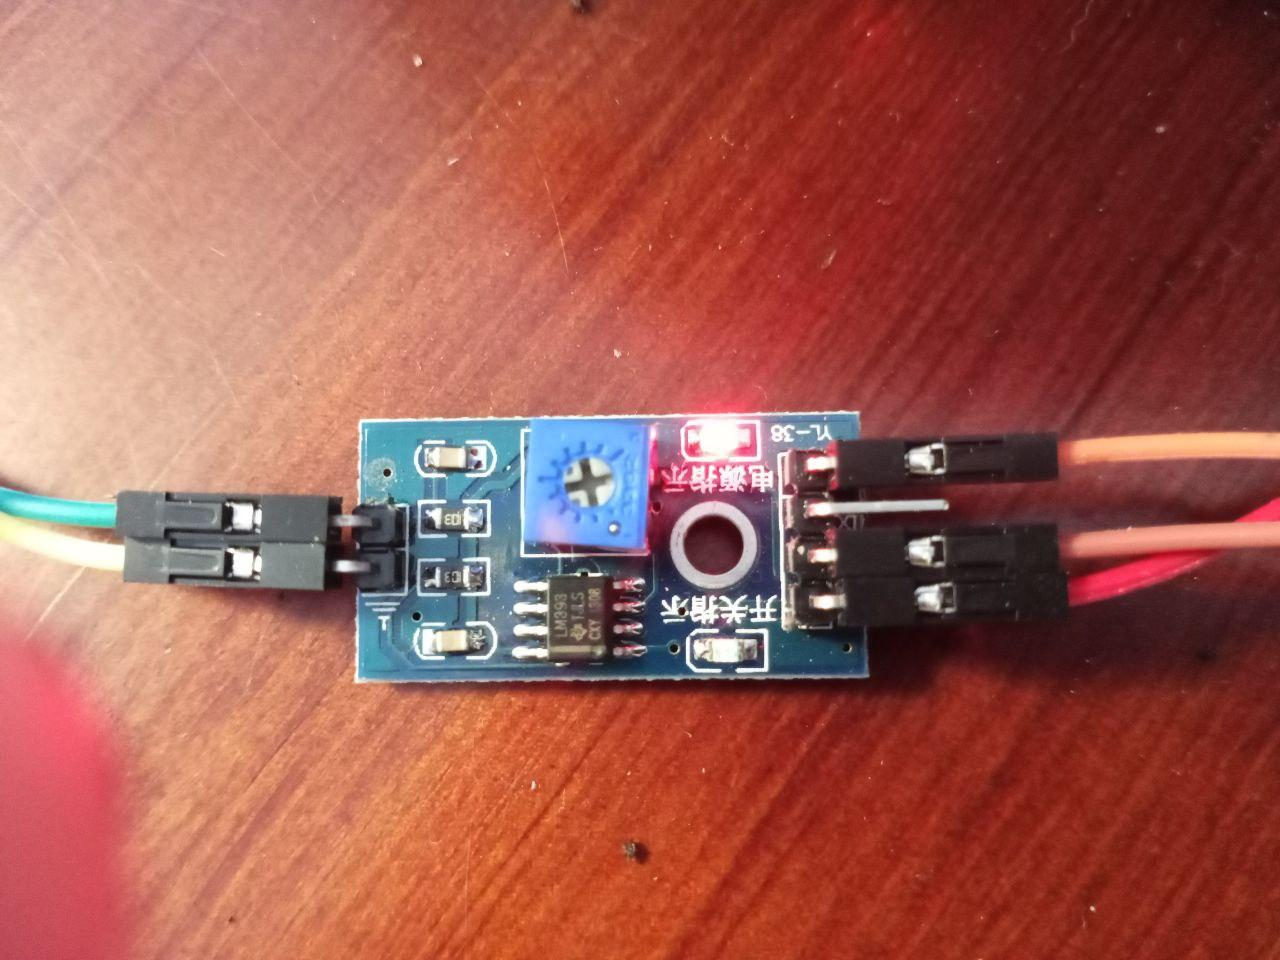
\includegraphics[width=0.35\textwidth]{fig/fc28-circuit2.jpg}
		\caption{LM293 comparator}
	\end{figure}

Now let's take a look at the script that is going to make the sensor work

\lstinputlisting{arduino/fc28.ino}

\subsubsection{Testing}

(Aquí iria un checklist y unas capturas de pantalla del output)

\subsection{Temperature sensor}
The DHT11 sensor\cite{dht11-manual} allows us to measure both temperature and humidity. It consists of an 8-bit microcontroller and two sensors tucked into a tiny blue plastic box. In this section we will see how to measure temperature, in the following section we will focus in measuring humidity.

\begin{figure}[H]
    \centering
    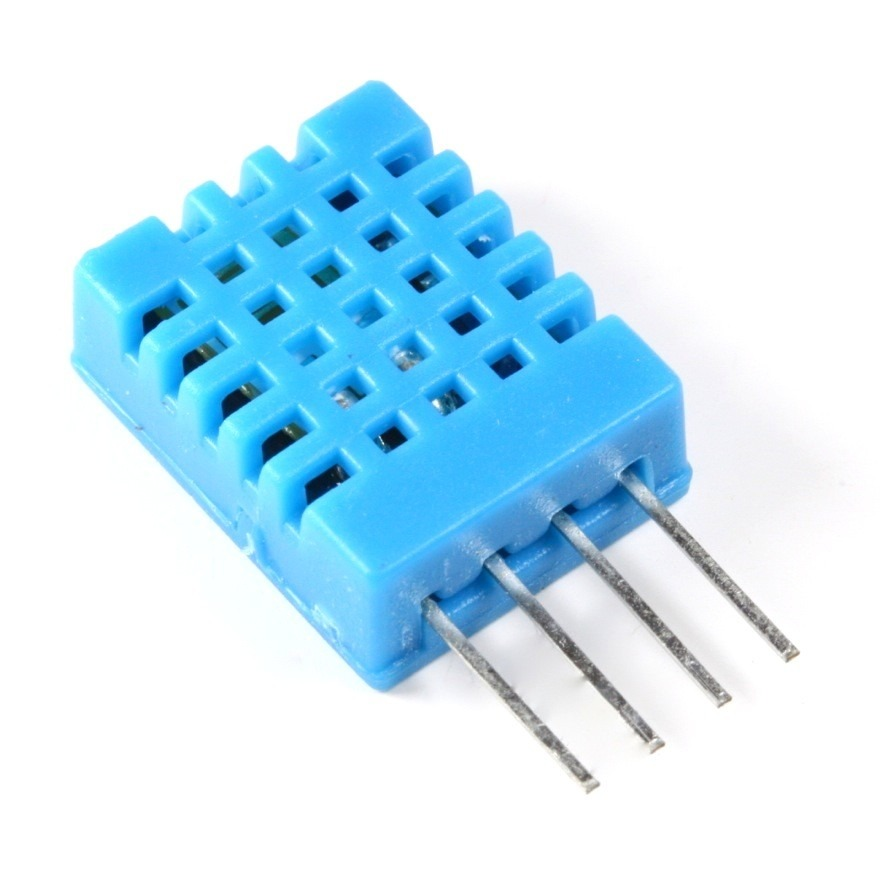
\includegraphics[width=0.3\textwidth]{fig/dht11.jpg}
    \caption{A DHT11 sensor}
    \label{fig:dht11}
\end{figure}

There are many applications for this sensor, it can be implemented as dehumidifier, for automatic control, data loggers or even weather stations. 

\subsection{Humidity sensor}

\subsection{LDR Sensor}
LDR (which stands for Light Dependent Resistor) sensor is a device used to detect light, it is a resistor made of semiconductor materials. This sensor is really sensitive to light. The stronger the light is, the lower the resistance. There are several uses for this kind of sensor, not only can you measure the value but also turn ON and OFF the light depending on the ambient light intensity.

\begin{figure}[htp]
    \centering
    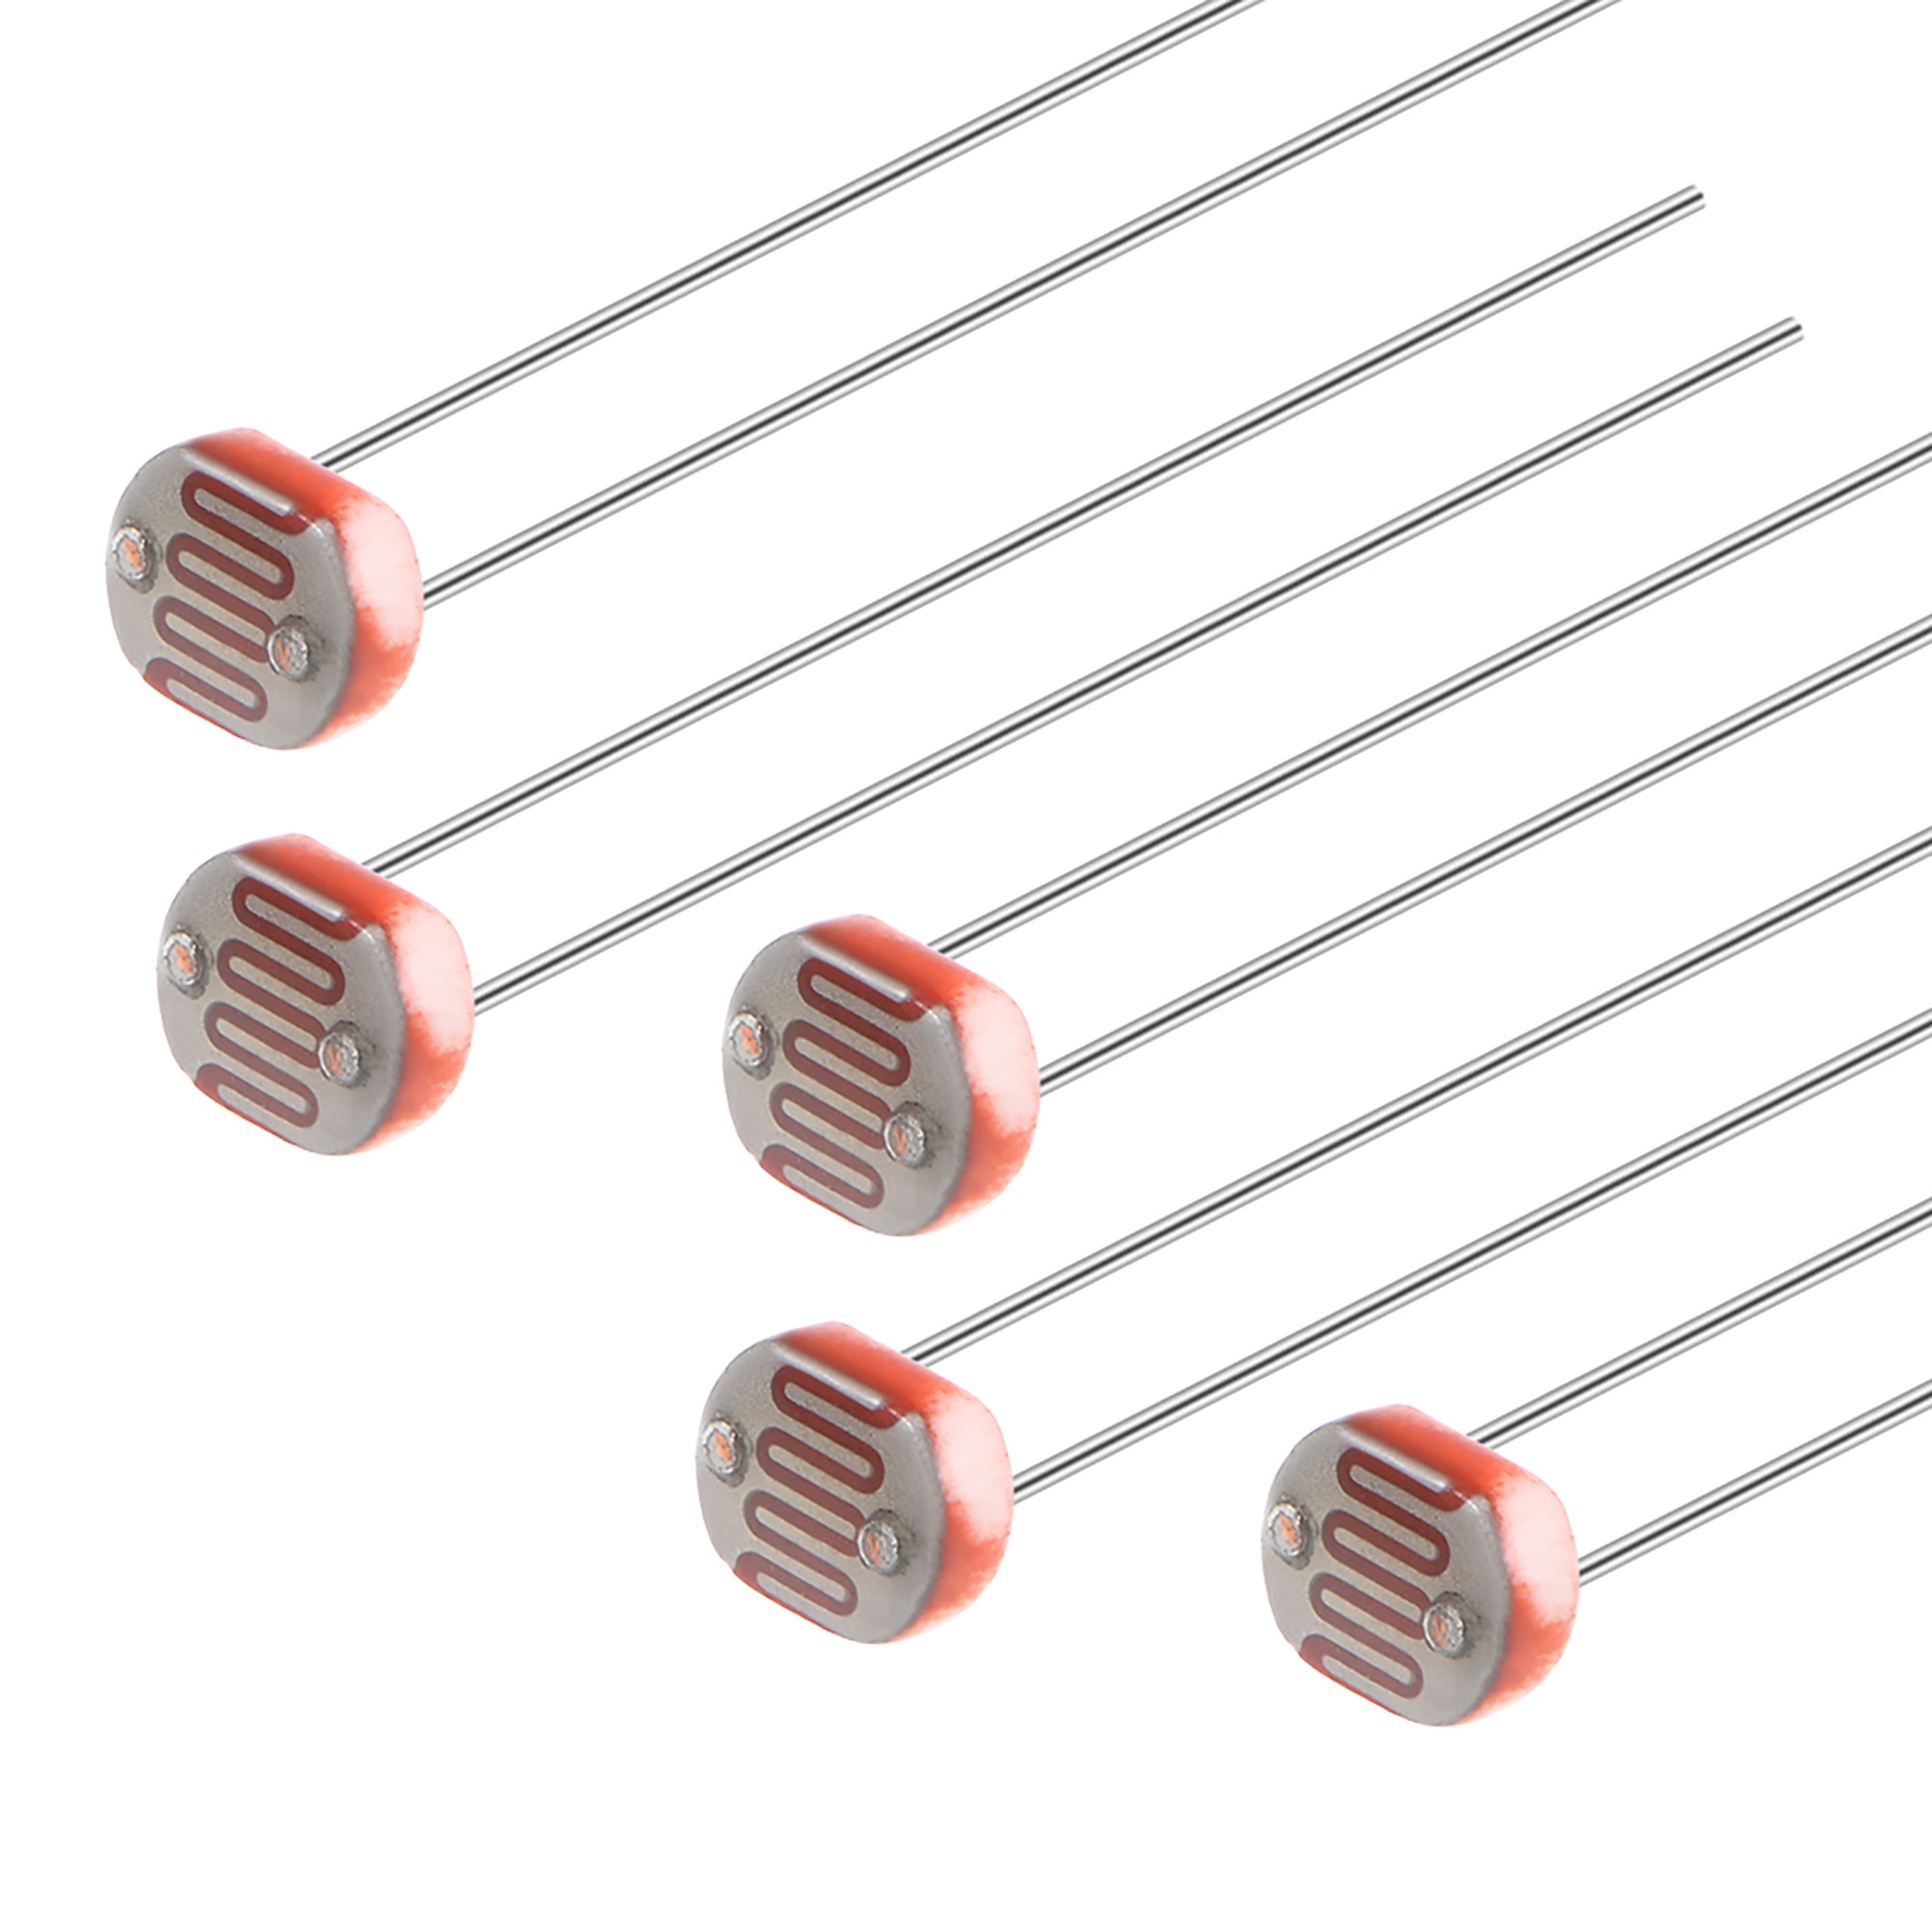
\includegraphics[width=0.35\textwidth]{fig/ldr.jpg}
    \caption{A LDR sensor}
    \label{fig:ldr}
\end{figure}

\subsubsection{Using the sensor}

\begin{figure}[H]
    \centering
    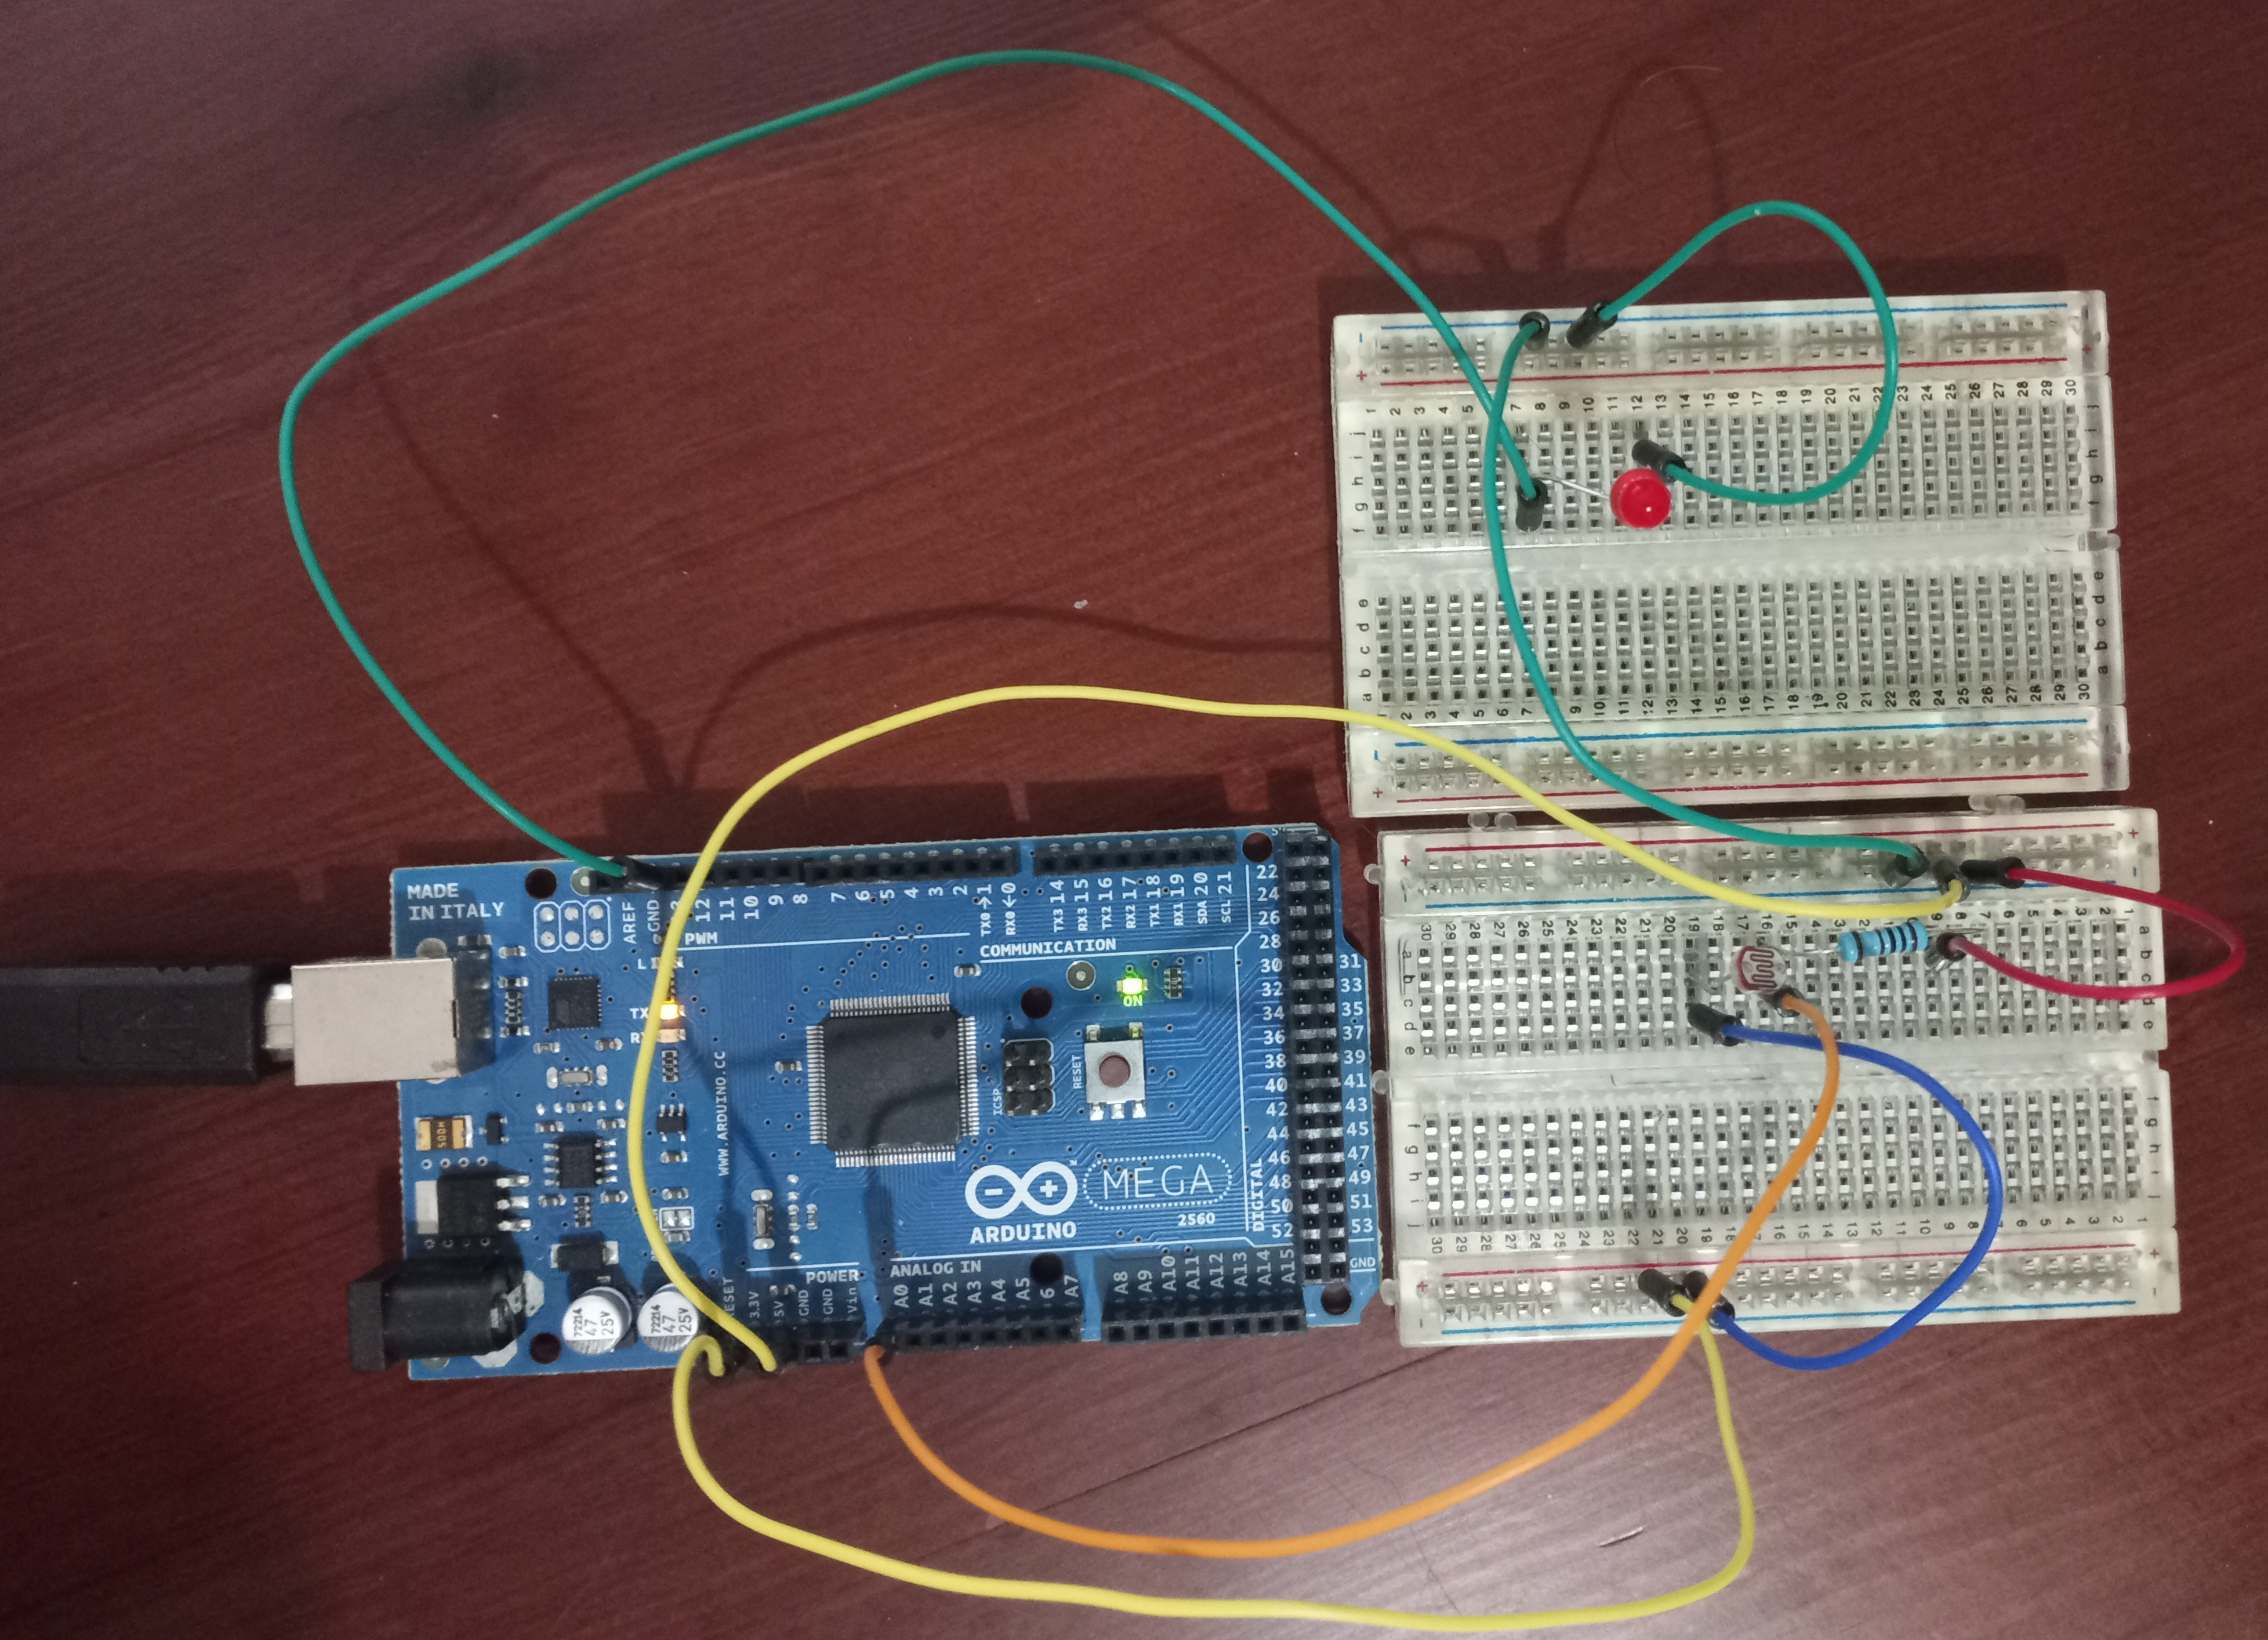
\includegraphics[width=0.5\textwidth]{fig/ldr-circuit.jpg}
    \caption{A LDR sensor}
    \label{fig:ldr}
\end{figure}


\lstinputlisting{arduino/ldr.ino}

\begin{figure}[H]
    \centering
    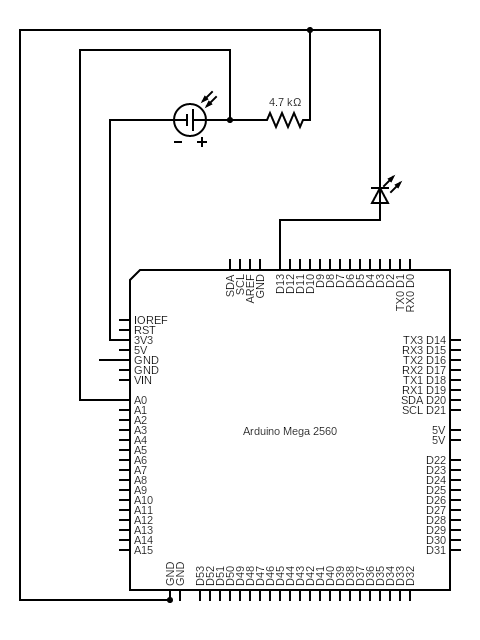
\includegraphics[width=0.7\textwidth]{fig/ldr-scheme-circuit.png}
    \caption{LDR circuit diagram}
    \label{fig:ldr}
\end{figure}


\subsubsection{Testing}

\subsection{PIR Motion sensor}
Another interesting asset that is about to be specified is the passive infrared motion sensor\cite{pir-guide}. In a nutshell, it can detect movement of objects that radiate infrared light, like humans. Because of this, and its eficiency and unexpensiveness, it's a sensor relatively common in security systems and it can have a lot of different applications in farming.

Some applications, besides of course the ones more related to security such as intruder detection, might include automatically switching ON and OFF several devices. See for example turning on a light when movement is detected, so the farmer or worker can forget about lighting and just focus in the main task.

\begin{figure}[H]
    \centering
    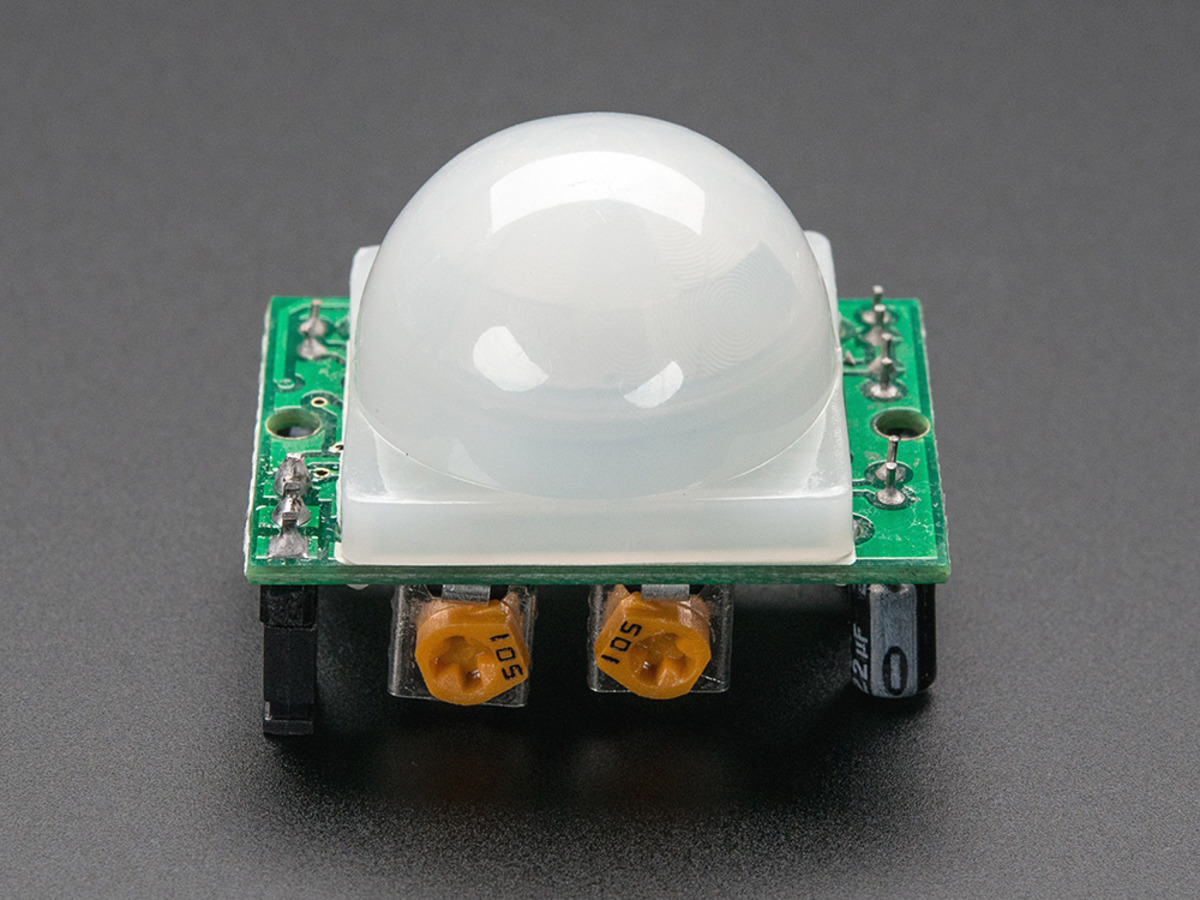
\includegraphics[width=0.35\textwidth]{fig/pir.jpg}
    \caption{Frontal view of PIR motion sensor}
    \label{fig:pir}
\end{figure}


There are several models of PIR motion sensors, but they all work pretty much in the same way. Let's see a bit of that.

They usually have a VCC pin, a GND pin and a digital output. The spherical form of the sensor improves the viewing angle. The PIR output can be connected to any digital pin of our Arduino board, the pin value will be set to "1" is the sensor detects any movement.

This is how a PIR sensor looks like upside down.

\begin{figure}[H]
    \centering
    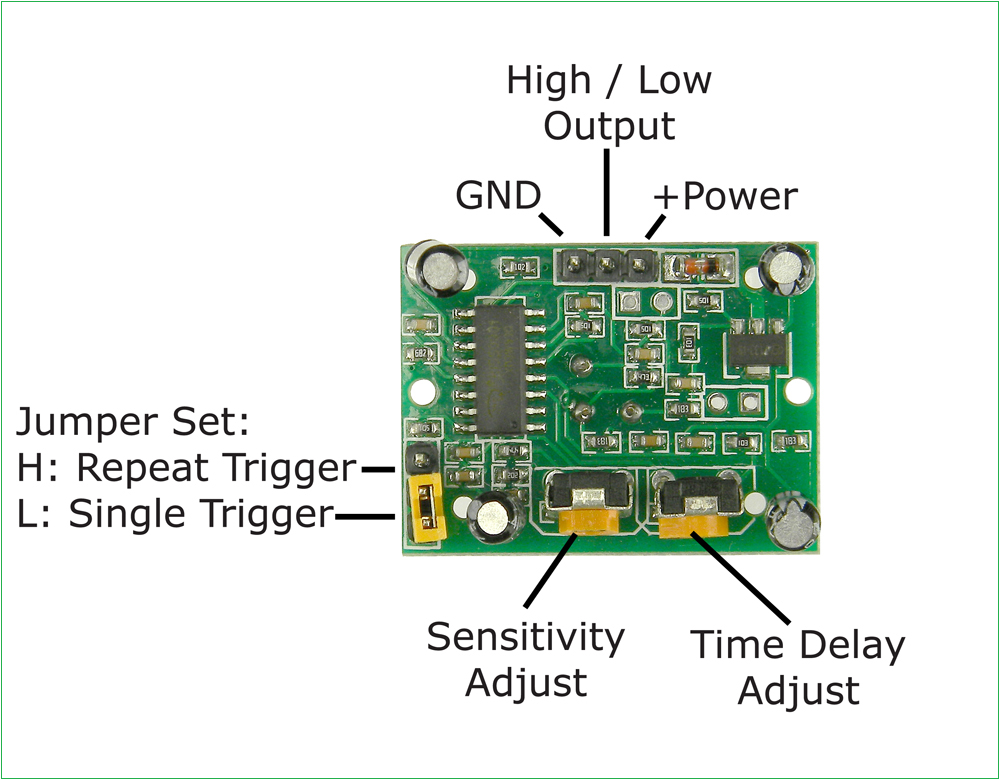
\includegraphics[width=0.6\textwidth]{fig/pir-upside-down.png}
    \caption{Upside down view of PIR motion sensor}
    \label{fig:pir-upsidedown}
\end{figure}

In this image, obtained from the Theory Circuit\cite{theory-circuit} blog, we can spot some parts of the sensor that are worth mentioning:

\begin{itemize}
	\item Time Delay Adjust. How long the output remains set to "1" after detecting motion.
	\item Sensitivity Adjust. Sets the detection range.
	\item Single Trigger Mode / Non-repeat Mode(L). Changes state every time a motion is detected. If we tried it in a practical example, we would see that the LED does not stay on when moving in front of the sensor, but turns on and off every second approximately. This is also called "non-retriggering". 
	\item Repeat Trigger Mode(H). For this position the sensor will turn on every time motion is derected and turn off a bit after the last motion. The way this works is by reseting the timer every single time a motion is detected. This is also called "retriggering". This mode is preferable for most applications, and it is the one we will be using in this project.
\end{itemize}

\subsubsection{Using the sensor}
Now that we have talked a bit about the behaviour of this PIR sensor, let's see how it can be implemented with a really simple example. In order to do so, let's start by taking a look at the circuit.

\begin{figure}[H]
    \centering
    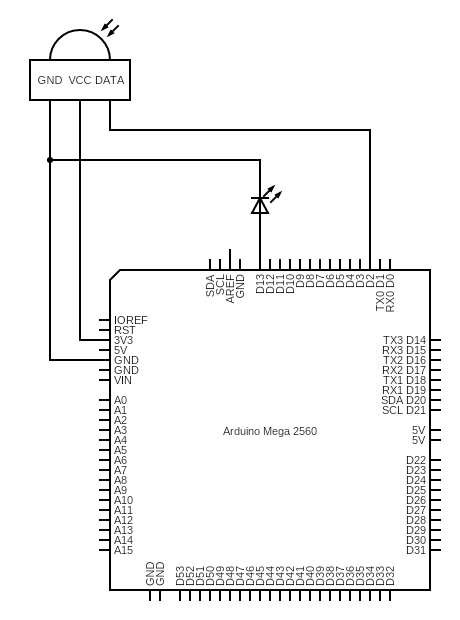
\includegraphics[width=0.7\textwidth]{fig/pir-scheme-circuit.png}
    \caption{Upside down view of PIR motion sensor}
    \label{fig:pir-scheme-circuit}
\end{figure}

In the circuit we have used a LED that will turn on when movement is detected. As it was mentioned before, the PIR is set to retriggering (H mode).

The output of the PIR sensor goes to pin 2 and then the pin 13 is connected to the LED. As it can be easily guessed, the LED pin will be set to OUTPUT mode and PIR pin to INPUT.

Here's a few lines of code for the circuit below.

\lstinputlisting{arduino/pir.ino}

\subsection{Ultrasonic sensor}

\lstinputlisting{arduino/ldr.ino}

\section{Implementation}
By this point we have a general view of how sensors work and how to test some of its basic features. As it was mentioned before, from this point on we will focus on implementing moisture and FC-28 sensors. In this section we will take a look at a similar code that suits better the specific needs of this prototype. Later on we will talk about how to send the information collected in this sensors to our farmOS system.

\section{Raspberry Pi server hosting}

\subsection{Introduction}
In this chapter we will walk through the installation and set up of a farmOS system in an Ubuntu Server hosted in a Raspberry Pi.


\subsection{Raspberry Pi configuration}
For our particular case we will be using a Raspberry Pi 4 Model B computer with 2GB RAM. The operating system that will be used is Ubuntu Server 20.
\section{Drupal and farmOS installation}


\section{Arduino and server communication}

\subsection{Ethernet shield}

\section{Conclusions}


